\section{Design Overview}\label{s:design}

\begin{figure*}
    \centering
    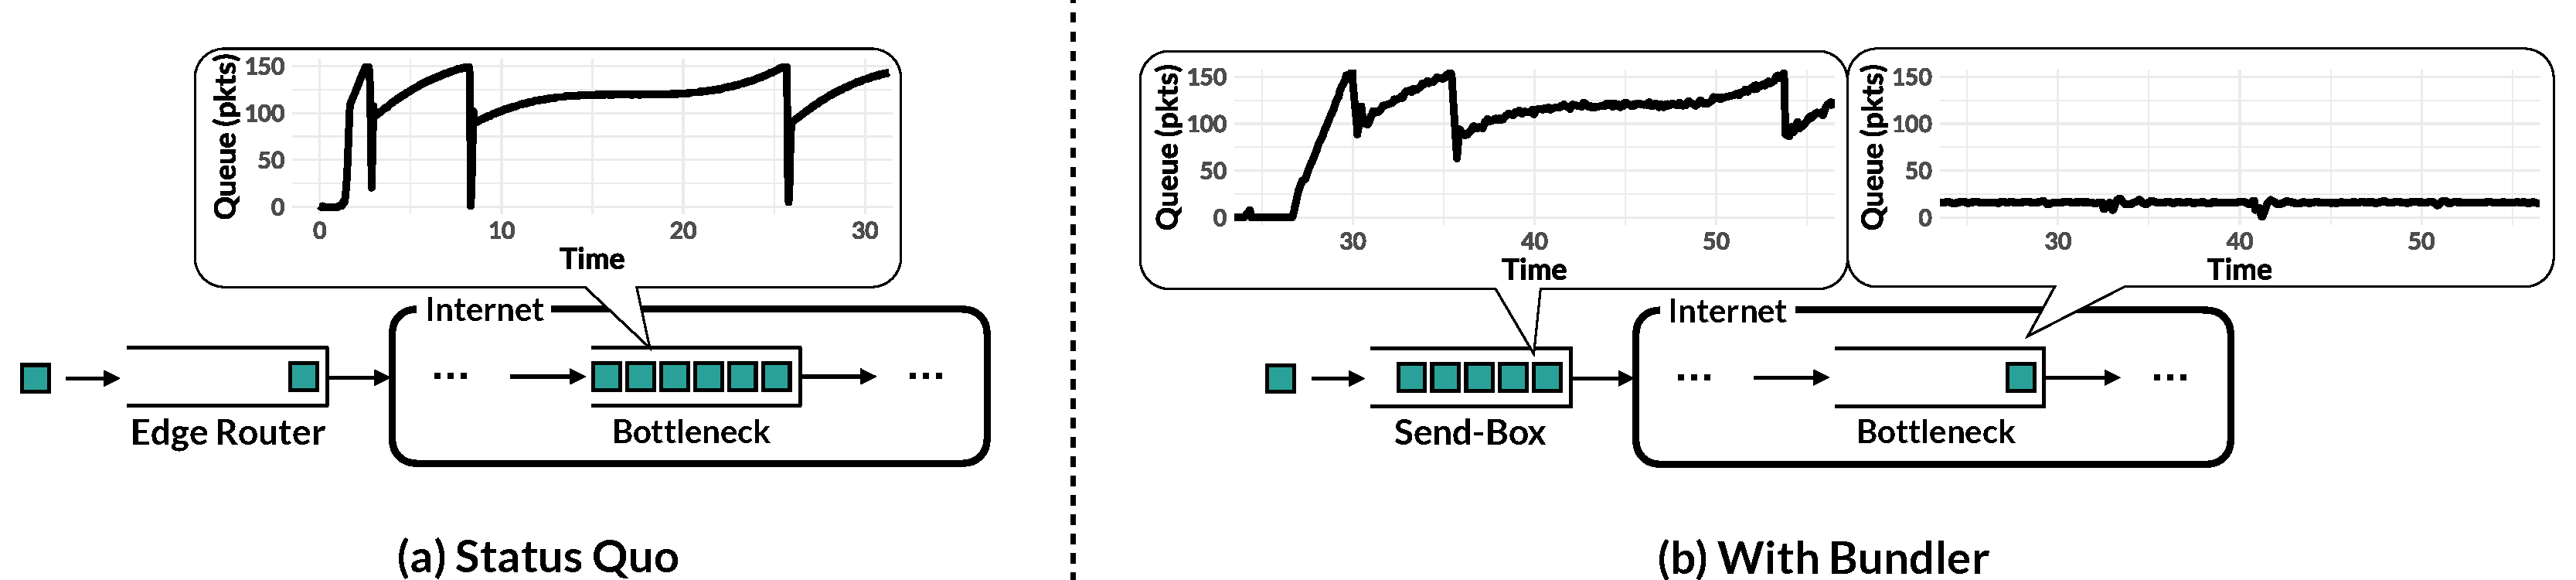
\includegraphics[width=\textwidth]{img/shift-bottleneck-combined}
    \caption{This illustrative example with a single flow shows how \name can take control of queues in the network. The plots show the trend in measured queueing delays at the relevant queue over time. The queue where delays build up can best make scheduling decisions, since it has the most choice between packets to send. Therefore, the \inbox \emph{shifts} the queues to itself to gain scheduling power.}\label{fig:design:shift-bottleneck}
\end{figure*}

\cut{
A \name must have the following properties:
\cut{ 
% these items could be considered implementation details
    \item It measures congestion control information from the network path.
    \item It enforces a pacing rate determined by a congestion control algorithm. The congestion control algorithm takes as input measurements from the network path, and returns an aggregate rate at which \name should send its component traffic.
}
\fc{mabye this starts too abruptly}
\begin{enumerate}
    \item It provides a mechanism for scheduling the packets comprising the aggregate.
    \item It must be deployable, therefore, it cannot rely on changes in end-hosts.
    \item It must be capable of deployments on the edge of a domain. Therefore, it must also scale to high link rates. As a result, it should not maintain per-connection state -- only per-aggregate state. \radhika{shorten}
\end{enumerate}
\radhika{Need a transition line: ``The rest of this section discusses .....''} 
}

%\subsection{Shifting the Queues}\label{s:design:shifting}

%The key insight of \name is that shifting the queues induced by a traffic bundle from the bottleneck to the sender's edge enables the sender to schedule the traffic within the bundle appropriately. Notice that \name can only shift (and therefore can only schedule) the component of the bottleneck queue which is self-inflicted by the traffic in a given bundle. 

Recall that in order to do scheduling, we need to move the queues from the network to the \name. 
In this section, we first describe our key insight for moving the in-network queues, and then explain our specific design choices. 

\subsection{Key Insight}

%The central idea behind \name is to make it a choke-point of a customer's traffic, such that queuing occurs at the \name where the customer can effectively enforce different scheduling policies, instead of occurring at the links in the middle of the network over which it has no control.  

A trivial strategy for inducing queuing at the \name is to throttle its outgoing rate. However, if this rate is made smaller than the bundle's share of bandwidth at the bottleneck link in the network, it can decrease throughput. Instead, the rate needs to be set such that the bottleneck link sees a small queue while remaining fully utilized (and the bundled traffic competes fairly in the presence of cross traffic). 
We make a simple, but powerful, observation: existing congestion control algorithms~\cite{nimbus, copa} perform exactly this calculation. 
Therefore, running such an algorithm at the \inbox to set a bundle's rate would reduce its self-inflicted queue at the bottleneck, shifting it to the \inbox instead, without impacting aggregate throughput. 
Note that each end host would continue running a traditional congestion control algorithm (\eg Cubic~\cite{cubic}, BBR~\cite{bbr}), as before, which are unaware of \name, but build queues at \inbox rather than in the network.

%In order to prevent under-utilization of the bottleneck links in the network, \name needs to occupy . 
%We make a simple, but powerful, observation: many congestion control algorithms perform exactly this calculation! 
%If we run an appropriate congestion control algorithm (as discussed later in \S\ref{s:design-choices}) at the \name, it will decide on a fair sending rate for each of its bundles as they compete with traffic from other domains. 
%Component flows of the bundles will then queue at the \name as their packets are sent at this rate.
%Since component flows, running traditional congestion control algorithms, will probe for bandwidth until they experience loss, they build queues at the \name instead of at the bottleneck.
%Since the \name now controls the queues corresponding to the traffic aggregate, it can schedule the packets of component flows. \radhika{needs fixing!}

Figure~\ref{fig:design:shift-bottleneck} illustrates this concept for a single flow traversing a bottleneck link in the network.\footnote{Details of the emulated network setup which resulted in the illustrated queue length time-series are in \S\ref{s:eval}.} Without \name, packets from the end hosts are queued in the network, while the queue at the edge is unoccupied. In contrast, a \name deployed at the edge is able to shift the queue to its \inbox.

%In the remainder of this section, we describe our design requirement and choices for \name. 
%\radhika{transition line}

%With this illustration of our overall design, the remainder of this section dives into our specific design choices, after highlighting some of their .



%The rest of this section discusses our design choices for \name (\S X), and ends with a note on the regime in which \name works the best (\S X)


% \subsection{Design Choices}
% \label{s:design-choices}

% Ease of deployability main guiding factor....

%\radhika{maybe add a subsection on choice of congestion control at \name. Potential outline below.}
\subsection{Design Choices}

Our key requirement of \emph{deployment and management ease} guides our design choices:

\paragraphn{(i)} \name requires no changes to the endhosts or to the routers in the network, making it independently deployable. 

\paragraphn{(ii)} \name maintains only per-bundle state, and no per-connection state (unless needed by a specific scheduling algorithm), allowing it to scale trivially with the number of in-bundle connections. 

\paragraphn{(iii)} The only persistent state maintained in the \name is the network condition (in the form of congestion signals) which can be naturally re-aquired, thus making it crash-resistant. 

%\name makes no changes to the headers of the packets traversing it, 
\paragraphn{(iv)} \name supports an entirely passive deployment model in which its component packets remain unmodified , 
ensuring no interference with other networking components in a packet's path~\cite{mboxbadness, ipoptions, quic}. We discuss this further in \an{forward pointer}.

\vspace{5pt}
\noindent We discuss specific design choices in more details below. 

\Para{Choice of congestion control algorithm} 
\name's congestion control algorithm must satisfy the following requirements: 

\paragraphi{(1) Ability to limit network queueing} \name must limit queueing in the network to move the queues to the \inbox. Therefore, congestion control algorithms which are designed to control delays are the appropriate choice. 
A loss-based congestion control algorithm, for example, is not a good choice for \name, since it would build up a queue at the network bottleneck and drain queues at the \inbox.

\paragraphi{(2) Detection of buffer-filling cross-traffic} Simultaneously, it is well-known that delay-controlling schemes (\eg Vegas~\cite{vegas}) compete poorly with buffer-filling loss-based schemes~\cite{nimbus, copa, timely}. Therefore, \name's congestion control must have a mechanism to detect the presence of such competing buffer-filling flows, and fall back to status quo performance. 

The emergence of such detection mechanisms in congestion control is recent: Copa~\cite{copa} detects whether the queue lengths it observes are consistent with its own fluctuations, and Nimbus\footnote{Nimbus is descibed in concurrently submitted work, paper \an{XX}} provides a more general mechanism which overlays a pattern on the sending rate and measures the cross traffic's crresponding response.
\name combines the two approaches, and use Copa's delay controller with Nimbus's cross traffic detection.
We detail the implementation of rate control at the \inbox in \an{forward pointer}.

\Para{Two-sided measurement of congestion signals}\label{s:design:twosided}
\begin{outline}
\1 Congestion control algorithms require network feedback from the receivers to measure congestion and adjust the sending rates accordingly. 
    \2 Conventional endhost-based implementations have used TCP acknowledgements for this.
    \2 However, this is not a good option for \name because: 
(i) it is incompatible with UDP, which is commonly used by video streaming applications \an{mention QUIC encrypted header?}, 
and (ii) it requires the reverse traffic to also pass through \name's \inbox, which may not always be the case.  
\1 There are three strategies for dealing with this
    \2 Proxy: terminate the connections, and collect the ACKs.
        \3 advantages: help midsize connections ramp up (traditional use to alleviate RTT unfairness)
        \3 disadvantages: must take responsibility for reliability. end-to-end principle violation. need to determine number of concurrently backlogged connections, in order to avoid head-of-line blocking.
        \3 so, it is important that the tunnelling mechanism be unreliable.
    \2 Unreliable L3 or L4(udp) tunnel. 
        \3 L4 tunnels \eg VXLAN~\cite{vxlan}.
        \3 L3 tunnels \eg (NV)GRE~\cite{nvgre}, IP-in-IP~\cite{ipinip}.
    \2 Independent measurements without packet modification (null-tunnel).
\1 We set aside terminating connections for the remainder of this discussion, but note that this approach is complementary with \name (see \S\ref{s:eval}).
\1 For the tunnel and null-tunnel cases, we propose:
\end{outline}

%Second, there can be significant differences in the RTT values between flows that are part of the same bundle, but belong to different receiving endhosts, which would make these values an unreliable congestion signal for the aggregated bundle. 
 Instead, \name's two-sided design allows measurement of congestion signals to be conducted solely between a \pair. We highlight the key features of our two-sided measurement technique below, and describe it in more detail in \S\ref{s:measurement}. 
 %\fc{train of thought is not as clear to me here}

\paragraphi{(1) Out-of-band feedback} 
%To conduct its measurements, the \inbox instead receives an explicit out-of-band \emph{feedback message} from the \outbox. 
The \outbox sends explicit out-of-band \emph{feedback messages} to the \inbox, which are used for measuring congestion signals. 
This out-of-band feedback mechanism is not only agnostic to the underlying protocol (be it TCP or UDP), but also side-steps the issue of enforcing that TCP acknowledgements pass through the same \inbox.

\paragraphi{(2) Infrequent measurements} Sending an out-of-band feedback message for every packet arriving at the \outbox would result in high communication overhead. Furthermore, conducting measurements on every outgoing packet at the \inbox would require maintaining state for each of them, which can be expensive, especially at high bandwidth-delay products. We, therefore, conduct measurements on a few sampled packets, at least once per RTT, which is sufficient for most congestion control algorithms~\cite{ccp}. 

\paragraphi{(3) Independent sampling} The \inbox and \outbox need to agree upon the set of sampled packets over which measurements will be conducted (to ensure overlap between the packets for which the \outbox generates feedback and the packets for which the \inbox maintains state). It is tempting to simply mark such packets at the \inbox. However, past studies~\cite{ipoptions, mboxbadness, quic} have shown how such strategies may fail in practice, as many deployed middleboxes have a tendency to drop or re-write packets with unfamiliar header fields. 
%Another option is to explicitly exchange coordination messages, but the overhead incurred by that would defeat the purpose of sampling packets. 
In the following section, we describe our technique to sample packets solely based on the hash computed over certain fields in the packet header, which allows the \inbox and the \outbox to independently sample the same set of packets.
